\documentclass[12pt]{article}
\usepackage{ficha}

\begin{document}

\ficha{Funções Racionais e Assíntotas}

\instrucoes{Resolve os exercícios, apresentando os cálculos. Apresenta os conjuntos-solução em notação de intervalos.}

\secao{Domínio e Zeros}{Determina o domínio e os zeros de cada função.}
\begin{exercicios}
  \item $f(x) = \dfrac{3}{x - 2}$
  \item $f(x) = \dfrac{x + 1}{x - 4}$
  \item $f(x) = \dfrac{2x - 6}{x + 3}$
  \item $f(x) = \dfrac{x^2 - 9}{x}$
  \item $f(x) = \dfrac{x}{x^2 - 4}$
  \item $f(x) = \dfrac{x^2 - 1}{x^2 + 1}$
  \item $f(x) = \dfrac{x - 2}{x^2 - 5x + 6}$
  \item $f(x) = \dfrac{1}{x} + \dfrac{1}{x - 1}$
\end{exercicios}

\secao{Funções do Tipo $a + \dfrac{b}{x - c}$}{Para cada função, indica as assíntotas, o domínio e o contradomínio, e esboça o gráfico.}
\begin{exercicios}
  \item $f(x) = \dfrac{1}{x} + 2$
  \item $f(x) = \dfrac{2}{x - 3}$
  \item $f(x) = 1 - \dfrac{3}{x + 1}$
  \item $f(x) = \dfrac{-1}{x - 2} - 4$
  \item Escreve $f(x) = \dfrac{2x + 1}{x - 1}$ na forma $a + \dfrac{b}{x - c}$ e indica as assíntotas.
  \item Escreve $f(x) = \dfrac{3x - 4}{x - 2}$ na forma $a + \dfrac{b}{x - c}$ e indica as assíntotas.
  \item Determina a expressão de uma função do tipo $a + \dfrac{b}{x - c}$ com assíntotas $x = 1$ e $y = 3$ que passa no ponto $(2, 5)$.
\end{exercicios}

\secao{Leitura de Gráficos}{O gráfico representa a função $f(x) = a + \dfrac{b}{x - c}$.}

\begin{center}
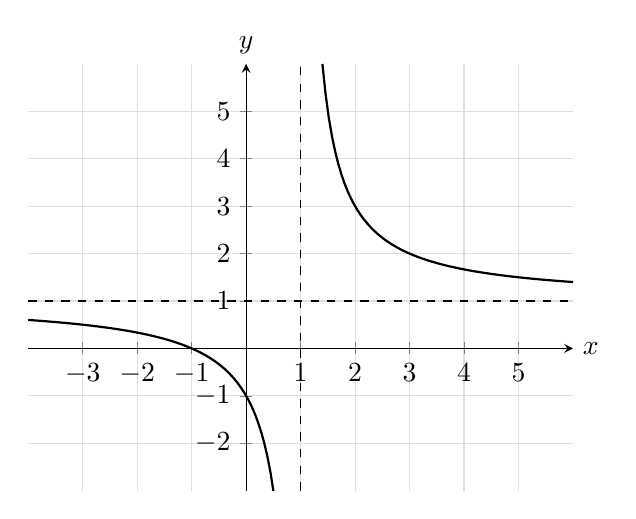
\begin{tikzpicture}
\begin{axis}[axis lines=middle, xmin=-4, xmax=6, ymin=-3, ymax=6, xtick={-3,...,5}, ytick={-2,...,5}, grid=both, grid style={gray!25}, width=8.5cm, height=7cm, xlabel=$x$, ylabel=$y$, every axis x label/.style={at={(ticklabel* cs:1)},anchor=west}, every axis y label/.style={at={(ticklabel* cs:1)},anchor=south}, restrict y to domain=-5:9]
  \addplot[thick, domain=-4:0.75, samples=80] {1 + 2/(x-1)};
  \addplot[thick, domain=1.4:6, samples=80] {1 + 2/(x-1)};
  \addplot[dashed, domain=-4:6] {1};
  \draw[dashed] (axis cs:1,-3) -- (axis cs:1,6);
\end{axis}
\end{tikzpicture}
\end{center}

\begin{exercicios}
  \item Indica as equações das assíntotas.
  \item Usando o ponto $(3, 2)$, determina $a$, $b$ e $c$.
  \item Indica o domínio e o contradomínio de $f$.
  \item Determina o zero de $f$ e a ordenada na origem.
  \item Resolve graficamente $f(x) > 1$.
\end{exercicios}

\secao{Equações Racionais}{Resolve, em $\R$.}
\begin{exercicios}
  \item $\dfrac{3}{x} = 6$
  \item $\dfrac{x + 2}{x - 1} = 4$
  \item $\dfrac{2}{x - 3} = \dfrac{1}{x}$
  \item $\dfrac{x}{x + 1} + \dfrac{2}{x} = 1$
  \item $\dfrac{x^2 - 4}{x - 2} = 0$
  \item $x + \dfrac{6}{x} = 5$
  \item $\dfrac{1}{x - 1} + \dfrac{1}{x + 1} = \dfrac{4}{x^2 - 1}$
\end{exercicios}

\secao{Inequações Racionais}{Resolve, em $\R$, usando um quadro de sinais.}
\begin{exercicios}
  \item $\dfrac{x - 2}{x + 3} > 0$
  \item $\dfrac{x + 1}{x - 4} \le 0$
  \item $\dfrac{2x - 6}{x} \ge 0$
  \item $\dfrac{x^2 - 9}{x - 1} < 0$
  \item $\dfrac{1}{x} < 2$
  \item $\dfrac{x + 3}{x - 1} \ge 2$
  \item $\dfrac{x^2 - x - 6}{x^2 - 1} \le 0$
\end{exercicios}

\secao{Desafios}{Resolve os problemas.}
\begin{exercicios}
  \item Uma torneira enche um tanque em 6 horas e outra em 3 horas. Quanto tempo demoram as duas juntas? (Escreve e resolve uma equação racional.)
  \item O custo médio de produção de $x$ peças é $C(x) = 5 + \dfrac{200}{x}$ euros por peça. Quantas peças é preciso produzir para o custo médio ser inferior a 7 euros? Interpreta a assíntota horizontal.
  \item Determina $k$ de modo que a função $f(x) = \dfrac{kx + 1}{x - 2}$ tenha assíntota horizontal $y = 3$.
  \item Mostra que o gráfico de $f(x) = \dfrac{x^2 - 1}{x - 1}$ é uma reta com um «buraco». Em que ponto?
\end{exercicios}

\end{document}
